\chapter{Arbeitspunkt-Regelung}\label{cha:apr}

Nachdem im letzten Kapitel die Modellierung des Gesamtsystems erläutert wurde, stellt sich nun die Frage, wie sich das System regeln lässt. Dabei geht es einerseits um die Regelung an den 4 Arbeitspunkten \siehe{\secref{sec:aps}} sowie um \traj n, die das \dpd\ von einem \ap\ in einen anderen überführen (siehe \charef{cha:traj}).

Beim Reglerentwurf wird dem Vorgehen vergangener Arbeiten gefolgt. 


\section{System-\lin\ und Analyse}%\label{sec:}

Das nicht-lineare System wird zunächst linearisiert, dessen \ewe\ analysiert, sowie auf Steuer- und Beobachtbarkeit überprüft.

\subsection{\lin}\label{sec:lin}

Da das \zrm\ des \spds s \eqref{eq:zrm} nicht-linear ist, muss es um jeden \ap\ linearisiert werden, bevor lineare Regelungsmethoden angewandt werden können. 
\begin{align}
	\mat{A} &= \left. \frac{\partial \vef(\vex,u_R)}{\partial \vex} \right|_{\vex=\vexr}  
		= \left. \begin{bmatrix}
		0 & 1 & 0 & 0 & 0 & 0 \\
		0 & \partiald{a_2(\vex)}{\xop} & \partiald{a_2(\vex)}{\phe} & \partiald{a_2(\vex)}{\phep} & \partiald{a_2(\vex)}{\phz} & \partiald{a_2(\vex)}{\phzp} \\
		0 & 0 & 0 & 1 & 0 & 0 \\
		0 & \partiald{a_4(\vex)}{\xop} & \partiald{a_4(\vex)}{\phe} & \partiald{a_4(\vex)}{\phep} & \partiald{a_4(\vex)}{\phz} & \partiald{a_4(\vex)}{\phzp} \\
		0 & 0 & 0 & 0 & 0 & 1 \\
		0 & \partiald{a_6(\vex)}{\xop} & \partiald{a_6(\vex)}{\phe} & \partiald{a_6(\vex)}{\phep} & \partiald{a_6(\vex)}{\phz} & \partiald{a_6(\vex)}{\phzp} \\
	\end{bmatrix} \right._{\vex=\vexr}  \\
	\mat{B} &= \left. \frac{\partial \vef(\vex_R,u)}{\partial u} \right|_{u=u_R}
	= \ve{b}(\vexr) = \begin{bmatrix}
		0 \\ b_2(\vexr) \\ 0 \\  b_4(\vexr) \\ 0 \\  b_6(\vexr)
	\end{bmatrix}
\end{align}
Somit ergeben sich für jeden \ap\ unterschiedliche Systemmatrizen \mat{A} und Eingangsmatrizen \ve{B}. Beim \bss\ fällt zusätzlich die zweite Zeile und die zweite Spalte (bis auf die 1) weg, da dort $a_2=0$ ist und keine Abhängigkeit von \xop\ besteht \siehe{\tabref{tab:abh}}, außerdem ist $b_2=1$.
Die Ausgangsmatrix \mat{C} ist immer gleich, da die Ausgangsgleichung \eqref{eq:hx} linear ist.


\subsection{Eigenwerte}

Anhand der \ewe\ können Aussagen über die Dynamik eines Systems getroffen werden. 
Das \bss\ hat aufgrund der zweifachen Integration des Eingangs \xopp\ stets zwei \ewe\ in 0. 
Mit den Apprich-Parametern ergeben sich folgende \ewe:

\begin{table}[htbp]
	\centering
	\caption{\ewe\ des \bss s (Parameter: Apprich)}
		\begin{tabular}[t]{cccc}
			\toprule
			\ape & \apz & \apd & \apv \\
			\midrule
			$0$	&	$0$	&	$0$	&	$0$	\\
			$0$	&	$0$	&	$0$	&	$0$	\\
			$-0.2972 +11.4177\iu$ &    $7.8028						$	&	  $6.8596							$	&   $11.1308$	\\
			$-0.2972 -11.4177\iu$ &   $-7.9367						$	&   $-7.2314					$		&  $-11.7251$	\\
			$-0.0418 + 4.8515\iu$ &   $-0.1858 + 7.0392\iu$	&  $-0.0669 + 7.8676\iu$	&  $  4.8089$	\\
			$-0.0418 - 4.8515\iu$ &   $-0.1858 - 7.0392\iu$	& $ -0.0669 - 7.8676\iu	$	&  $ -4.8926$	\\
			\bottomrule
		\end{tabular}
	\label{tab:ewappr}
\end{table}
Im \ap\ 1 ergeben sich zwei konjugiert-komplexe Polpaare, die sich physikalisch mit der Schwingung der beiden Pendel begründen lassen. Sie befinden sich aufgrund der Dämpfung in der linken s-Halbebene, es ist der einzige stabile \ap. \ap\ 2 und 3 besitzen jeweils ein konjugiert-komplexes Polpaar, da dort das erste \bzw zweite Pendel nach unten zeigt und damit \qq{stabil} ist. Der Realteil ist bei \ap\ 3 deutlich kleiner, was auf die geringere Dämpfung des zweiten Pendelgelenks zurückzuführen ist (siehe \tabref{tab:parappr}). Aufgrund der Instabilität des anderen Pendels ergibt sich jeweils ein positiv reeller \ew. In \ap\ 4 stehen beide Pendel oben, weswegen es dort zwei \ewe\ in der rechten s-Halbebene gibt.

\begin{table}[htbp]
	\centering
	\caption{\ewe\ des \bss s (Parameter: Ribeiro)}
		\begin{tabular}[t]{cccc}
			\toprule
			\ape & \apz & \apd & \apv \\
			\midrule
				$0$	&	$0$	&	$0$	&	$0$	\\
				$0$	&	$0$	&	$0$	&	$0$	\\
				$-174.3727$						&	$-172.9211$	&	$-173.2473$						&	$-175.4362$	\\
				$-0.3493$							&	$-0.3494$		&	$0.3471$							&	$0.3471$	\\
				$-0.6385 + 7.1578\iu$	&	$6.7715$		&	$-0.6443 + 7.2040\iu$	&	$6.7469$	\\
				$-0.6385 - 7.1578\iu$	&	$-7.6900$ 	&	$-0.6443 - 7.2040\iu$ &	$-7.6570$ \\
			\bottomrule
		\end{tabular}
	\label{tab:ewribe}
\end{table}

Mit den neuen Parametern (Ribeiro) ergibt sich ein anderes Bild (siehe \tabref{tab:ewribe}).
Bei \ap\ 1 und 2 verschwindet ein Polpaar, welches dem ersten Pendel zugeordnet wurde. Ein sehr schneller \ew\ kommt hinzu, außerdem ein langsamer reeller, der bei \ap\ 3 und 4 positiv ist. 
Die Ursache für diese Änderung liegt vermutlich in der Modellierung der \crb\ (siehe \secref{sec:crb}). Bei der \lin\ um die Ruhelage wird die Annäherungsfunktion der \mrm{signum}-Funktion um 0 linearisiert, wo sie sehr steil ist. Dies resultiert in einer sehr hohen Dämpfung. Daher ist es sinnvoll, die \crb\ der Pendelstäbe für den AP-Reglerentwurf zu vernachlässigen.
Wird die \crb\ zu 0 gesetzt, ergeben sich prinzipiell ähnliche Werte wie in \tabref{tab:ewappr}.


\subsection{Steuerbarkeit und Beobachtbarkeit}

Voraussetzung für eine Regelung ist die Steuerbarkeit des Systems. Diese kann für lineare Systeme oder linearisierte Systeme an einem \ap\ mit dem Steuerbarkeitskriterium nach \textsc{Kalman} überprüft werden \cite{AdamyRT2}. Außerdem sollte ein System beobachtbar sein, falls nicht alle Zustände bekannt sind und daher über einen Beobachter ermittelt werden.

Das \spds\ (\bss) ist an allen 4 \ap en vollständig steuer- und beobachtbar.


\section{Regelungskonzept}

Die Aufgabe eines Reglers \bzw einer (Vor-)Steuerung ist es nun, anhand der Messgrößen $\vey=(\xo\ \phe\ \phz)^{\transp}$ \eqref{eq:hx} eine geeignete Steuerspannung $U_{\mrm{Steuer}}$ an den Motor vorzugeben. Dabei teilt sich die Steuerung/Regelung in mehrere Schritte auf. 


\subsection{Zustandsregler}

Die \aprg\ wird mit einem \zsr\ realisiert ($u=-K \vexd$). 
Dieser regelt ein System grundsätzlich in den Ursprung, es muss also noch eine Zustandstransformation durchgeführt werden. 
Für jeden der \ap e \secref{sec:aps} wird der Zustand, der für den \zsr\ die Endlage darstellt, vorher von den Messgrößen abgezogen. 
Nach Berechnung der Stellgröße und Schätzung des Zustands wird der \ap\ wieder dazu addiert.

Die Verstärkung $K$ wird durch Lösen des LQ-Problems bestimmt \cite{AdamyRT2}. Parameter für den Entwurf sind somit die positiv-definite Matrix 
$\mat{Q}=\diaga \left(\begin{matrix} q_1 & q_2 & q_3 & q_4 & q_5 & q_6 \end{matrix}\right)$
 zur Bewertung der Zustände und $R$ für die Stellgröße. 

Für jeden \ap\ muss ein eigener Regler entworfen werden, da jedem \ap\ ein anderes lineares System zugrunde liegt (siehe \secref{sec:lin}).
Der AP-Regler ist somit nur in der Umgebung der Ruhelage gültig und kann zu große Abweichungen aufgrund der Nichtlinearität möglicherweise nicht ausregeln.
Außerdem sind für jeden \ap\ andere Güteparameter \mat{Q} und $R$ optimal. Die systematische simulative Optimierung erfolgt in \secref{sec:x0qr}.

Das Lösen der \emph{Riccati}-Gleichung und die Berechnung von $K$ für alle \ap e erfolgt automatisiert in \ml.


\subsection{Zustandsermittlung}

Ein \zsr\ benötigt zur Regelung zu jedem Zeitpunkt die Information aller Zustände \vex\ \eqref{eq:vex} des Systems. Beim \spds\ werden die drei Zustände \xo, \phe\ und \phz\ gemessen. Deren Ableitungen, die Zustände \xop, \phep\ und \phzp\ müssen noch ermittelt werden. Dabei wird von drei Möglichkeiten ausgegangen, die in der Simulation miteinander verglichen werden können:
\begin{enumerate}
	\item Zustandsmessung
	\item Beobachter
	\item Differenzieren 
\end{enumerate}
Am Versuchsstand erfolgt die Zustandsermittlung durch einen \beob.

\subsubsection{\zm}
Bei der \zm\ wird von einer idealen Messung aller Zustände ausgegangen, \dah $\vexd=\vex$. 
Diese Variante wird in der Simulation meist zuerst eingesetzt, um die Regelung des Systems besser beurteilen zu können und spezielle Probleme durch die \ze\ im Nachhinein analysieren zu können.
Am realen Versuchsstand kann diese Methode nicht eingesetzt werden.

\subsubsection{\beob}\label{subsec:beob}
Der Schätzzustand $\vexd$ wird durch einen \emph{Luenberger-Beobachter} ermittelt. 
Dieser \qq{simuliert} ein lineares Schätzsystem (\mat{A}, \mat{B}, \mat{C}) und regelt Unterschiede in den Ausgangsgrößen \vey\ und \veyd\ mit der \beob-Matrix \mat{L} aus \cite{AdamyRT2}. 
Wie beim \zsr\ muss auch hier die Auslegung für jeden \ap\ separat erfolgen.
Damit gilt allerdings auch, dass der \beob\ nur in der Nähe dieser Ruhelage gültig ist, bei zu großen Abweichungen kann er aufgrund der \lin\ die Zustände nicht mehr richtig schätzen.

\mat{L} wird in dieser Arbeit mittels Polplatzierung ausgelegt. 
Einflussparameter sind somit die Pole des Beobachters $\vep_b$\,. 
Diese sollten üblicherweise weiter links liegen als die Pole des geregelten Systems $\vep_r$\,. 
Sie können aber nicht beliebig weit links liegen, da sonst Messrauschen verstärkt wird.

In \cite{brehl} werden sie beispielsweise hintereinander auf der negativen reellen Achse verteilt:
	\[
	\vep_b=\begin{bmatrix}
		-40 & -41 & -42 & -43 & -44 & -45
	\end{bmatrix}
\]
Im Allgemeinen ist es aus oben genannten Gründen sinnvoll, die \beob-Pole in Abhängigkeit der Pole des geschlossenen Regelkreises zu definieren.
Bei \cite{chang} werden sie nach
	\[
	\vep_b = \vep_r - 25
\]
bestimmt, wodurch allerdings komplexe \beob-Pole möglich sind. In dieser Arbeit werden sie daher meist folgendermaßen berechnet:
	\[
	\vep_b = \Re\left\{{\vep_r \cdot 5}\right\}
\]
%Im \ml-Code kann die Definition geändert werden und die verschiedenen Auslegungen miteinander verglichen werden.

Neben dem Messvektor \vey\ ist auch die Stellgröße $u$ Eingang des \beob. 
Dafür könnte man direkt die geforderte Stellgröße des \zsr\ $u_\mrm{reg}$ verwenden.
Allerdings wird letztere bei bestimmten Regelabweichungen häufig deutlich über der maximalen Stellgröße liegen, sodass die Ausgangsstellgröße spätestens beim Motor begrenzt wird.
Wenn der Beobachter dies nicht mitbekommt und daher sein System mit der unbegrenzten Regler-Stellgröße simuliert, gibt es zwangsläufig Abweichungen zwischen \beob-System und realem System.
Der Zustand wird nicht mehr richtig geschätzt, folglich ergibt sich ein schlechteres Regelverhalten, bis hin zur Instabilität.

Aus diesen Gründen ist es sinnvoll, eine Vorsteuerung zu implementieren \siehe{\secref{sec:motvorst}}, die die Stellgröße schon vor der Ausgabe an den Motor begrenzt und die tatsächliche Stellgröße zurück an den \beob\ gibt, sodass dieser das reale System besser nachbilden kann.
Somit weicht die Stellgröße nur noch bei Stellgrößeneinbrüchen anderer Art \siehe{\secref{subsec:dcMotor}} ab.


\subsubsection{\diff}
Die übrigen Zustände werden durch Differentiation der Messgrößen und \evtl Tiefpass-Filterung gebildet:
\begin{align}
	\vexd=\begin{bmatrix}
		1	&	0	&	0	\\
		\ddt	&	0	&	0	\\
		0	&	1	&	0	\\
		0	&	\ddt	&	0	\\
		0	&	0	&	1	\\
		0	&	0	&	\ddt	\\
	\end{bmatrix} \vey  = \begin{bmatrix}
		\xom \\ \ddt \xom \\ \phem \\ \ddt \phem \\ \phzm \\ \ddt \phzm
	\end{bmatrix}
\end{align}
In der Simulation kam es hierbei zu Problemen, da für eine möglichst glatte und fehlerfreie Differentiation eine kleine Schrittweite notwendig ist, außerdem hat sich die Simulation in manchen Fällen aufgehängt. Daher wird diese Variante in dieser Arbeit nicht weiter verfolgt.

Trotzdem sei angemerkt, dass diese Möglichkeit am realen Versuchsstand in Kombination mit einer sinnvollen Filterung der Messgrößen und den Ableitungen möglicherweise Vorteile gegenüber einem Beobachter darstellt. 
Es ist kein Einschwingen der Startzustände nötig, es gibt keine Probleme bei Stellgrößenstörungen und die Differentiation muss nicht für jeden \ap\ einzeln ausgelegt werden.


\subsection{Vorsteuerung F/a und a/v-Regler}

Ist der AP-Regler nach dem \bss\ ausgelegt, gibt dieser als Stellgröße eine Sollbeschleunigung \asoll\ für den Schlitten vor. 
Aus dieser muss die geforderte Motorkraft bestimmt werden.
Sie kann zum Großteil mit einer Vorsteuerung bestimmt werden, die Differenz wird mit einem Geschwindigkeitsvergleich ausgeregelt.
Diese Aufteilung in einen \ap regler am einfacheren \bss\ und eine unterlagerte Geschwindigkeitsregelung, um der störenden Reibung am Schlitten zu begegnen, hat sich in vergangenen Arbeiten als sinnvoll herausgestellt.

\subsubsection{a/v-Regler}
Die Sollgeschwindigkeit \vsoll\ wird durch Integration von \asoll\ berechnet.
Dadurch kann ein Soll/Ist-Vergleich mit der realen \bzw geschätzten Schlittengeschwindigkeit \xop\ durchgeführt werden.
Die Regelung wird durch einen P-Regler umgesetzt:
	\[
	\fav= \kpv (\vsoll-\xopd)
\]
Brehl \cite{brehl} ging für \kpv\ beispielsweise von 500 aus, während im \sm-Modell von \cite{chang} 150 verwendet wird.
Der Parameter scheint am realen Modell einen starken Einfluss auf die Stabilität und ein mögliches \qq{Ratterverhalten} zu haben.
In dieser Arbeit wird ein Wert von 150 angenommen und der Parameter nicht weiter untersucht, da es in der Simulation meist nur geringe Abweichungen von der Sollgeschwindigkeit gibt.

Als problematischer stellte sich hingegen ein möglicher \emph{Windup-Effekt} heraus: 
Ist die Sollbeschleunigung größer als wegen der \sgb\ tatsächlich erreicht werden kann, wird \vsoll\ immer weiter aufintegriert und damit auch \fav, obwohl die Motorkraft bereits maximal ist. 
Wenn das System wieder aus der \sgb\ ist und die Vorsteuerungskraft eigentlich das Vorzeichen wechselt, ist der I-Anteil noch vorhanden und muss erst abgebaut werden.
In dieser Zeit übersteigt \fav\ daher \fvorst\ und die Stellgröße geht somit praktisch in die falsche Richtung, was die Regelung sehr schnell instabil werden lassen kann.
Aus diesem Grund wird \asoll\ vor der Integration mit einem Sättigungsglied auf 
	\[
	a_\mrm{soll,max}=\frac{\fmax}{m}
\] 
begrenzt.

\subsubsection{\vorst\  (M,C,D)}
Der \avr\ alleine könnte die Schlittenkraft zwar regeln, allerdings kann der Hauptteil der Kraft mit einer Vorsteuerung bestimmt werden, wodurch die Dynamik besser ist.
Die Vorsteuerung besteht im Wesentlichen aus der Trägheitskraft, da bei reiner Betrachtung des Schlittens $\fsoll=m_0 \asoll$ gilt. 
Wenn davon ausgegangen wird, dass die Reibungsparameter hinreichend genau bestimmt wurden, kann auch die Reibung des Schlittens kompensiert werden.
Während \cite{brehl} nur die Trägheitskraft vorsteuerte, wird in \cite{chang} die Vorsteuerung folgendermaßen berechnet:
	\[
	\fvorst=m \asoll + \Fco \, \sign{\vsoll} + d_0 \xop
\]

\subsubsection{\vorst\  mit Systemgleichung}
Auch die obige Gleichung bestimmt die benötigte Kraft nicht exakt, da es je nach Winkellage der Pendel rückwirkende Kräfte auf den Schlitten gibt.
Man kann daher einen Schritt weiter gehen und die benötigte Kraft zur Beschleunigung des Schlittens direkt aus der entsprechenden Bewegungsgleichung herleiten. 
Auch wenn am realen Versuchsstand die Beschleunigung aufgrund von Ungenauigkeiten nicht exakt mit \asoll\ übereinstimmt, wird dem \avr\ dadurch weitere \qq{Arbeit abgenommen}.

Die Beziehung zwischen der Schlittenbeschleunigung und der Kraft am Schlitten wird durch die zweite Zustandsgleichung \eqref{eq:zrmF} beschrieben:
\begin{align}
	a=\xopp=f_2(\vex,F)
	\label{eq:xpp}
\end{align}
Diese Gleichung kann leicht nach der Kraft umgestellt werden:
\begin{align}
	\fsoll=\frac{\asoll-a_2(\vex)}{b_2(\vex)}
\end{align}
Damit diese Berechnung für beliebige Systemparameter und somit unterschiedliche Funktionen $a_2$ und $b_2$ erfolgen kann, wird die Bestimmung der Vorsteuerkraft in dieser Arbeit symbolisch in \ml\ automatisiert.

\subsubsection{Ermittlung reale Beschleunigung}
In \secref{subsec:beob} wurde erläutert, dass es sinnvoll ist, die reale Stellgröße an den \beob\ zu geben.
Im folgenden Vorsteuerungsblock (\secref{sec:motvorst}) wird die vor dem Motor begrenzte Kraft \freal\ zurückgegeben, da die \sgb\ \fmax\ bekannt ist.
Ist der \beob\ allerdings am \bss\ ausgelegt, geht er bei der Stellgröße von der Beschleunigung aus.
Somit muss aus \freal\ zunächst \areal\ bestimmt werden.

Dies kann ähnlich wie bei der Kraftvorsteuerung durch die Trägheit geschehen, was allerdings ungenau ist und der \beob\ demzufolge von einer falschen Eingangsgröße ausgeht.
Daher wird die Ermittlung der tatsächlichen Beschleunigung wie im vorigen Abschnitt über die Systemgleichung vorgenommen.
Es gilt \eqref{eq:xpp}.



\subsection{Motor Vorsteuerung}\label{sec:motvorst}






\section{Simulationsmodell in \Simulink}



\section{Implementierung in \Matlab}



\section{Anfangswert-Tests}\label{sec:x0test}

\newcommand{\scalee}{0.48}

\begin{figure}
	\centering
	\subfloat[\apaz]{ \includegraphics[scale=\scalee]{Bilder/Parameter neu (Ribeiro) Creg off/AP2.pdf} }
	\hfil
	\subfloat[\apad]{	\includegraphics[scale=\scalee]{Bilder/Parameter neu (Ribeiro) Creg off/AP3.pdf} }
	\\
	\subfloat[\apave]{ \includegraphics[scale=\scalee]{Bilder/Parameter neu (Ribeiro) Creg off/AP41.pdf} }
	\hfil
	\subfloat[\apavz]{ \includegraphics[scale=\scalee]{Bilder/Parameter neu (Ribeiro) Creg off/AP42.pdf} }
	\caption{Maximalabweichungen -- Vergleich QR-Parameter (System Ribeiro)}
	\label{fig:qrvglrib}
%\vspace{15pt}
\end{figure}




\section{QR Parameter Tests}\label{sec:x0qr}



\section{System Parameter Tests}\label{sec:x0sys}

System Ribeiro

\newcommand{\scaleq}{0.62}
\begin{figure}
	\centering
	\subfloat[\apaz]{ \includegraphics[scale=\scaleq]{Bilder/SysParam Variation/m1/AP2.pdf}	}
	\hfil
	\subfloat[\apad]{	\includegraphics[scale=\scaleq]{Bilder/SysParam Variation/m1/AP3.pdf}	}
	\\
	\subfloat[\apave]{ \includegraphics[scale=\scaleq]{Bilder/SysParam Variation/m1/AP41.pdf} }
	\hfil
	\subfloat[\apavz]{ \includegraphics[scale=\scaleq]{Bilder/SysParam Variation/m1/AP42.pdf}	}
	\caption{Maximale Startwerte -- Variation $m_1$}
	\label{fig:sysvarm1}
	%\vspace{15pt}
\end{figure}

\begin{figure}
	\centering
	\subfloat[\apaz]{ \includegraphics[scale=\scaleq]{Bilder/SysParam Variation/m2/AP2.pdf}	}
	\hfil
	\subfloat[\apad]{	\includegraphics[scale=\scaleq]{Bilder/SysParam Variation/m2/AP3.pdf}	}
	\\
	\subfloat[\apave]{ \includegraphics[scale=\scaleq]{Bilder/SysParam Variation/m2/AP41.pdf} }
	\hfil
	\subfloat[\apavz]{ \includegraphics[scale=\scaleq]{Bilder/SysParam Variation/m2/AP42.pdf}	}
	\caption{Maximale Startwerte -- Variation $m_2$}
	\label{fig:sysvarm2}
	%\vspace{15pt}
\end{figure}

